\chapter{TinyDES}

TinyDES là một phiên bản thu nhỏ của chuẩn mã hóa DES. TinyDES
là mã hóa khối theo mô hình Feistel, kích thước khối là 8 bit, kích
thước khóa cũng là 8 bit. Mỗi vòng khóa con có độ dài 6 bit.

\begin{figure}[ht]
    \centering
    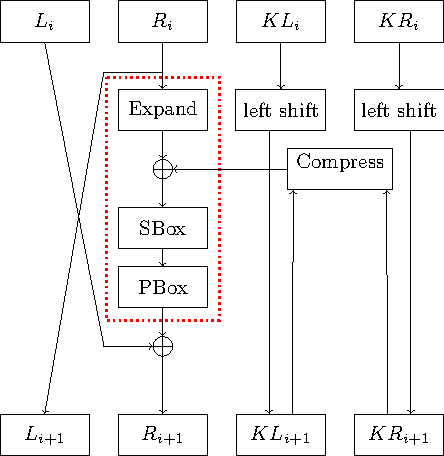
\includegraphics{../pics/tinydes/blocky.pdf}
    \caption{Một vòng TinyDES}
\end{figure}

Mã TinyDES khá đơn giản. Theo mô hình Feistel, khối đầu vào 8 bit được chia thành
hai nửa trái phải 4 bit. Nửa phải sẽ đi qua các hàm Expand, SBox và PBox, sau đó
XOR với nửa trái để được nửa phải mới. Còn nửa trái mới là nửa phải cũ. Tóm lại 
công thức mô hình Feistel là
\[L_{i+1} = R_i, \quad R_{i+1} = F(R_i, K_i) \oplus L_i\]
với $i = 0, 1, 2$ tương ứng 3 vòng.

Chúng ta cần các động tác sau:

\begin{enumerate}
    \item Expand: mở rộng và hoán vị $R_i$ từ 4 bit lên 6 bit. Giả sử 4 bit
    của $R_i$ là $b_0 b_1 b_2 b_3$ thì kết quả sau khi Expand là $b_2 b_3 b_1
    b_2 b_1 b_0$;
    \item SBox: gọi 6 bit đầu vào là $b_0 b_1 b_2 b_3 b_4 b_5$. Khi đó ta tra
    cứu theo bảng SBox với $b_0 b_5$ chỉ số \textbf{hàng}, $b_1 b_2 b_3 b_4$ chỉ
    số \textbf{cột}. Nói cách khác bảng SBox có 4 hàng, 16 cột. Kết quả của SBox
    là một số 4 bit;
    \item PBox: là hàm hoán vị 4 bit $b_0 b_1 b_2 b_3$ thành $b_2 b_0 b_3 b_1$
\end{enumerate}

Như vậy, hàm $F$ của mô hình Feistel đối với mã TinyDES là
\[F(R_i, K_i) = PBox(SBox(Expand(R_i) \oplus K_i))\]

Để sinh khóa con cho 3 vòng, khóa ban đầu được chia
thành hai nửa trái phải lần lượt là $KL_0$ và $KR_0$. 
TinyDES thực hiện như sau:

\begin{enumerate}
    \item Vòng 1: $KL_0$ và $KR_0$ được dịch vòng trái 1 bit để được $KL_1$ và $KR_1$;
    \item Vòng 2: $KL_1$ và $KR_1$ được dịch vòng trái 2 bit để được $KL_2$ và $KR_2$;
    \item Vòng 3: $KL_2$ và $KR_2$ được dịch vòng trái 1 bit để được $KL_3$ và $KR_3$.
\end{enumerate}

Khi đó, khóa $K_i$ ở vòng thứ $i$ (với $i = 1, 2, 3$) là hoán vị và nén 8 bit
của $KL_i$ và $KR_i$ lại thành 6 bit. Đặt 8 bit khi ghép $KL_i \Vert KR_i$ là 
$k_0 k_1 k_2 k_3 k_4 k_5 k_6 k_7$, kết quả là 6 bit $k_5 k_1 k_3 k_2 k_7 k_0$.